% Para compilar correr: "make" e dpois "make clean"
\documentclass{report}
\usepackage[T1]{fontenc} % Fontes T1
\usepackage[utf8]{inputenc} % Input UTF8
\usepackage[backend=biber, style=ieee]{biblatex} % para usar bibliografia
\usepackage{csquotes}
\usepackage[portuguese]{babel} %Usar língua portuguesa
\usepackage{blindtext} % Gerar texto automaticamente
\usepackage[printonlyused]{acronym}
\usepackage{hyperref} % para autoref
\usepackage{graphicx}

\bibliography{bibliografia}


\begin{document}
%%
% Definições
%
\def\titulo{PROJETO 2}
\def\data{14/07/2021}
\def\autores{Gonçalo Silva, Samuel Teixeira, Pompeu Costa, Hugo Hadden}
\def\autorescontactos{(103244) goncalolsilva@ua.pt, (103325) samuelsteixeira@ua.pt,\\
 (103294) pompeu@ua.pt,(98449) hugohadden@ua.pt}
\def\versao{VERSAO FINAL}
\def\departamento{Departamento de Eletrónica, Telecomunicações e
Informática}
\def\empresa{Universidade de Aveiro}
\def\logotipo{ua.pdf}
%
%%%%%% CAPA %%%%%%
%
\renewcommand{\contentsname}{Índice}
\begin{titlepage}

\begin{center}
%
\vspace*{50mm}
%
{\Huge \titulo}\\ 
%
\vspace{10mm}
%
{\Large \empresa}\\
%
\vspace{10mm}
%
{\LARGE \autores}\\ 
%
\vspace{30mm}
%
\begin{figure}[h]
\center
\includegraphics{\logotipo}
\end{figure}
%
\vspace{30mm}
\end{center}
%
\begin{flushright}
\versao
\end{flushright}
\end{titlepage}

%%  Página de Título %%
\title{%
{\Huge\textbf{\titulo}}\\
{\Large \departamento\\ \empresa}
}
%
\author{%
    \autores \\
    \autorescontactos
}
%
\date{\data}
%
\maketitle

\pagenumbering{roman}

%%%%%%%%%%%%%%%%%%%%%%%%%%%%%%%% RESUMO %%%%%%%%%%%%%%%%%%%%%%%%%%%%%%%%
\begin{abstract}
Este projeto foi realizado no âmbito da cadeira \ac{labi} do 1º ano do \ac{miect}. 
Consiste na criação de um sistema que permita criar músicas através da composição 
de pedaços/ excertos de música. Para além disso, também tivemos de fazer
este mesmo relatório em que explicamos o projeto: objetivo, motivação, a
metodologia utilizada, resultados, análise e conclusões.
Na metodologia, será relatado em pormenor o código feito para construir este projeto
, bem como o modo de funcionamento, testagem e comandos git feitos para tal.
Nos resultados, será mostrado o fruto de todo o nosso código que é a aplicação web a funcioanr.
Por fim, nas conclusões, retira-se o que se alcançou com este projeto, o que aprendemos,
o quão útil este projeto é para compreendermos esta matéria da cadeira de LABI e o 
quão interessante foi realizá-lo.
\end{abstract}

%%%%%%%%%%%%%%%%%%%%%%%%%%%%%%%% Agradecimentos %%%%%%%%%%%%%%%%%%%%%%%%%%%%%%%%
% Segundo glisc deveria aparecer após conclusão...
\renewcommand{\abstractname}{Agradecimentos}
\begin{abstract}
Queremos agradecer a todos os professores da cadeira de \ac{labi} por nos terem
dado um trabalho interessante, que nos ajudou a compreender os conceitos
lecionados nas aulas.
\end{abstract}


\tableofcontents
% \listoftables     % descomentar se necessário
% \listoffigures    % descomentar se necessário


%%%%%%%%%%%%%%%%%%%%%%%%%%%%%%%
\clearpage
\pagenumbering{arabic}

%%%%%%%%%%%%%%%%%%%%%%%%%%%%%%%% INTRODUÇÃO %%%%%%%%%%%%%%%%%%%%%%%%%%%%%%%%%

\chapter{Introdução}
\label{chap.introducao}

Introduz o tema, apresenta a motivação e finalmente a estrutura.

O objetivo deste trabalho é criar uma aplicação web que permita criar músicas através da 
composição de excertos de música. A Interface web, tem três páginas, na primeira são 
listadas as músicas existentes, na segunda os excertos e na terceira, um gerador de 
músicas, que permita ao utilizador criar a sua própria música, baseada nos excertos 
disponíveis. Além disso, nas duas primeiras páginas, é possível o utilizador visualizar a
informação acerca de cada música/ excerto, sendo até possível ouvi-lo.

Este documento está dividido em quatro capítulos.
Depois desta introdução,
no \autoref{chap.metodologia} é apresentada a metodologia seguida,
no \autoref{chap.resultados} são apresentados os resultados obtidos,
sendo estes discutidos no \autoref{chap.analise}.
Finalmente, no \autoref{chap.conclusao} são apresentadas
as conclusões do trabalho.

%%%%%%%%%%%%%%%%%%%%%%%%%%%%%%%%% METODOLOGIA %%%%%%%%%%%%%%%%%%%%%%%%%%%%%%%%%

\chapter{Metodologia}
\label{chap.metodologia}
Descreve os métodos utilizados para obtenção de resultados.

Neste esqueleto de relatório aproveitamos este capítulo para exemplificar
como se usam alguns elementos de {\LaTeX}.

Explicar as funções e métodos usados

\section{Gerador de Músicas}
\label{sec:songEngine}

\subsection{Função checkSong}
\label{ssec:checkSong}

\section{Servidor Cherrypy}
\label{sec:serCherrypy}

\subsection{Função principal}
\label{ssec:princfunc}

\section{Interface Web}
\label{sec:Inte_Web}

\subsection{JavaScript}
\label{ssec:JS}

\section{Git}
\label{sec:git}
As funcionalidades do git foram muito utilizados neste projeto, desde a simples sincronização 
de ficheiros e código, até à criação, junção e gestão de branches (\textbf{\autoref{fig:git_c}} e 
\textbf{\autoref{fig:git_d}}). 
\cite{git}

\begin{figure}[!h]
\center 
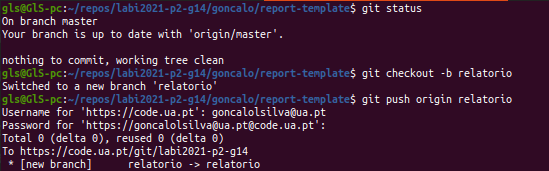
\includegraphics[height=100pt]{img/git_1.png}
\caption{Exemplo da criação de branches (criação branch relatorio)}
\label{fig:git_c}
\end{figure}

\begin{figure}[!h]
\center 
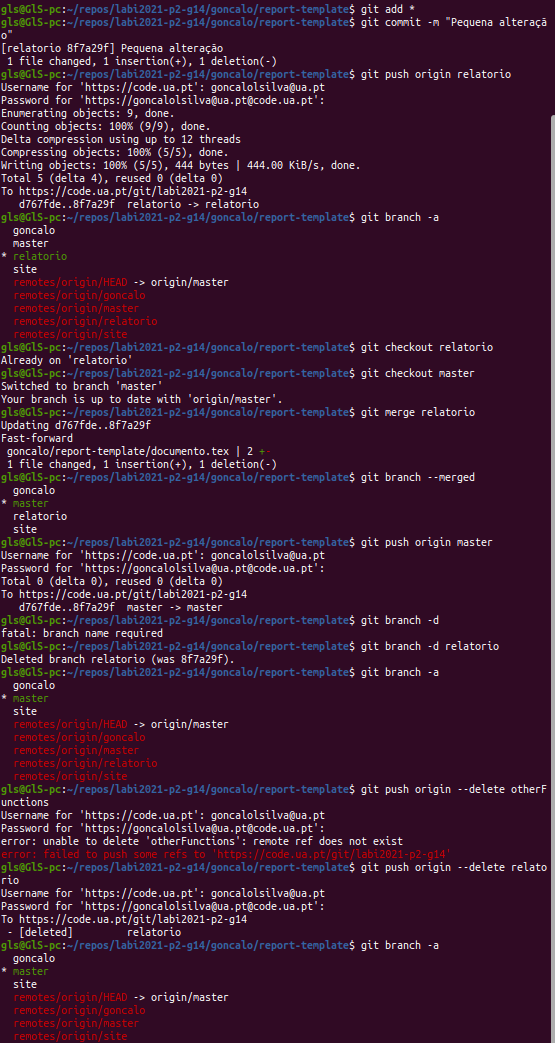
\includegraphics[height=220pt]{img/git_2.png}
\caption{Exemplo da eliminação de branches (eliminação branch relatorio)}
\label{fig:git_d}
\end{figure}

\section{Code UA}
\label{sec:codeua}
As funcionalidades do Code UA forneceram bastante ajuda ao desenvolvimento do projeto, 
desde a própria visualização dos branches disponíveis, bem como a própria gestão e 
visualização do código, até à criação de funcionalidades a serem desenvolvidas e bugs 
a serem resolvidos. Pode visualizar o projeto no Code UA, através do 
link: http://code.ua.pt/projects/labi2021-p2-g14
\cite{codeua}

\section{Exemplos}

\subsection{Utilização de acrónimos}
\label{sec.util}
Esta é a primeira invocação do acrónimo \ac{ua}.
E esta é a segunda: \ac{ua}.


Outras duas referências a \ac{miect}
e \ac{miect}.

\subsection{Referências bibliográficas}
Informação relativa à estrutura formal de um relatório pode ser obtida
na página do \ac{glisc}\cite{glisc}.

Como foi apresentado na \autoref{sec.util}...

%%%%%%%%%%%%%%%%%%%%%%%%%%%%%%%%% RESULTADOS %%%%%%%%%%%%%%%%%%%%%%%%%%%%%%%%%

\chapter{Resultados}
\label{chap.resultados}
Descreve os resultados obtidos com este relatório.

\section{Funcionamento}
\label{sec:funcionamento}

A \autoref{fig:iniciar_server} mostra o comando de inicio do servidor.
Mostrar o servidor em funcionamento

\section{Testes}
\label{sec:testes}

Os testes às funcionalidades foram feitos através de testes funcionais e unitários criados para 
o efeito. Estes testes são corridos usando a ferramenta pytest incorporada no python. 
Os testes albergam três ficheiros, o ficheiro test\_songEngine.py e test\_func\_songEngine.py, 
testam as funções de criação e obtenção de músicas do servidor, através de testes unitários e
funcionais. O ficheiro test\_app.py, testa as funcionalidadesdo servidor cherrypy.

É possível correr estes testes através do comando \textbf{"python3 -m pytest"}, como nos mostra 
a \autoref{fig:testes}.

\begin{figure}[ht]
\center 
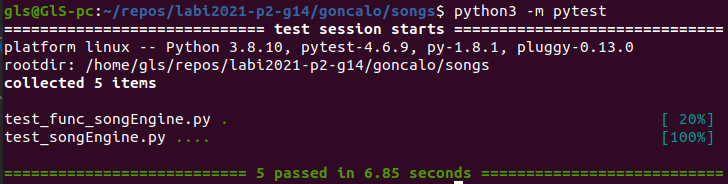
\includegraphics[height=90pt]{img/pytest.png}
\caption{Exemplo de execução dos testes ao songEngine}
\label{fig:testes}
\end{figure}

%%%%%%%%%%%%%%%%%%%%%%%%%%%%%%%%% ANÁLISE %%%%%%%%%%%%%%%%%%%%%%%%%%%%%%%%%

\chapter{Análise}
\label{chap.analise}
Analisa os resultados.
Mostrar que as músicas foram criadas e ficou tudo correto

%%%%%%%%%%%%%%%%%%%%%%%%%%%%%%%%% CONCLUSÕES %%%%%%%%%%%%%%%%%%%%%%%%%%%%%%%%%
\chapter{Conclusões}
\label{chap.conclusao}
Com este trabalho, conseguimos solidificar o nosso conhecimento em várias linguagens, como HTML, JavaScript, CSS e 
Python, bem como outras funcionalidades, como o cherrypy, pytest e operações com músicas (wave).
Apesar das adversidades, acreditamos que o trabalho foi conseguido com sucesso, criámos uma aplicação 
web com as funcionalidades referidas e todas as características necessárias para tal, utilizando os recursos que 
nos foram fornecidos e auxiliando a sua compreensão com este relatório.

\chapter*{Contribuições dos autores}
Resumir aqui o que cada autor fez no trabalho.
Usar abreviaturas para identificar os autores,
por exemplo AS para António Silva.
No fim indicar a percentagem de contribuição de cada autor.

%%%%%%%%%%%%%%%%%%%%%%%%%%%%%%%%% ACRÓNIMOS %%%%%%%%%%%%%%%%%%%%%%%%%%%%%%%%
\chapter*{Acrónimos}
\begin{acronym}
\acro{ua}[UA]{Universidade de Aveiro}
\acro{miect}[MIECT]{Mestrado Integrado em Engenharia de Computadores e Telemática}
\acro{lei}[LEI]{Licenciatura em Engenharia Informática}
\acro{labi}[LABI]{Laboratórios de Informática}
\acro{glisc}[GLISC]{Grey Literature International Steering Committee}
\end{acronym}


%%%%%%%%%%%%%%%%%%%%%%%%%%%%%%%%% BIBLIOGRAFIA %%%%%%%%%%%%%%%%%%%%%%%%%%%%%%%%
\printbibliography

\end{document}
